%\documentclass[singlecolumn, 9pt, conference]{IEEEtran}
\documentclass[10pt, conference]{IEEEtran}
%\documentclass[11pt, conference]{IEEEtran}
%\documentclass[onecolumn,11pt]{IEEEtran}
\usepackage{latexsym,amssymb,amsmath} % for \Box, \mathbb, split, etc.
\usepackage{citesort} % sorts citation numbers appropriately
\usepackage[]{graphicx} % use this when importing ps- and eps-files
%\usepackage{lscape}
\usepackage{setspace}
\usepackage{color}
\usepackage[T1]{fontenc}
\usepackage{courier}
\definecolor{mygray}{rgb}{0.8,0.8,0.8}
\usepackage{listings}
\lstset{
  language=C,                  % choose the language of the code
  %numbers=left,                   % where to put the line-numbers
  numbers=left,                   % where to put the line-numbers
  stepnumber=1,                   % the step between two line-numbers.        
  numbersep=5pt,                  % how far the line-numbers are from the code
  backgroundcolor=\color{mygray},  % choose the background color. You must add \usepackage{color}
  showspaces=false,               % show spaces adding particular underscores
  showstringspaces=false,         % underline spaces within strings
  showtabs=false,                 % show tabs within strings adding particular underscores
  tabsize=2,                      % sets default tabsize to 2 spaces
  frame=single, 		  %  adds a frame around the code
  captionpos=b,                   % sets the caption-position to bottom
  %basicstyle=\footnotesize	  % the size of the fonts that are used for the code
  breaklines=true,                % sets automatic line breaking
  breakatwhitespace=true,         % sets if automatic breaks should only happen at whitespace
  title=\lstname,                 % show the filename of files included with \lstinputlisting;
  basicstyle=\small\ttfamily % Font
}



% *** GRAPHICS RELATED PACKAGES ***
%
\ifCLASSINFOpdf
  % \usepackage[pdftex]{graphicx}
  % declare the path(s) where your graphic files are
  % \graphicspath{{../pdf/}{../jpeg/}}
  % and their extensions so you won't have to specify these with
  % every instance of \includegraphics
  % \DeclareGraphicsExtensions{.pdf,.jpeg,.eps}
\else
  % or other class option (dvipsone, dvipdf, if not using dvips). graphicx
  % will default to the driver specified in the system graphics.cfg if no
  % driver is specified.
  % \usepackage[dvips]{graphicx}
  % declare the path(s) where your graphic files are
  % \graphicspath{{../eps/}}
  % and their extensions so you won't have to specify these with
  % every instance of \includegraphics
  % \DeclareGraphicsExtensions{.eps}
\fi
%
\usepackage{algorithm}

\usepackage[noend]{algorithmic}
\usepackage{array}
%\usepackage{mdwmath}
\usepackage{subfigure}

%\topmargin   -28mm    %bottom margin 30mm
%\oddsidemargin  -11mm    %left & right margin 15mm text sizes
%\textwidth  190mm
%\textheight 258mm
%\columnsep  8.00mm
%\parindent  3.5mm

%\setstretch{0.8}
\setstretch{1.08}



\renewcommand{\algorithmicrequire}{\textbf{Input:}}
\renewcommand{\algorithmicensure}{\textbf{Output:}}
\floatname{algorithm}{Procedure:}
\begin{document}
%
% paper title
% can use linebreaks \\ within to get better formatting as desired
\title{Comparision of Binding Approaches of Scheduled Multiphase Application to Multicore Architecture}
% author names and affiliations
% use a multiple column layout for up to three different
% affiliations
%\author{\IEEEauthorblockN{Aryabartta Sahu, M. Balakrishnan, Preeti Ranjan Panda }
%\IEEEauthorblockA{Department of Computer Science and Engineering, Indian  Institute of Technology, Delhi\\
%Hauz Khas, New Delhi, India, 110016, Email: \{asahu,mbala,panda\}@cse.iitd.ac.in
%}
%}

%\author{\IEEEauthorblockN{Bhoopendra Kumar, Aryabartta Sahu }
%\IEEEauthorblockA{Department of Computer Science and Engg. IIT Guwahati, India\\
% Emails : bhoopendrakumar1@gmail.com, asahu@iitg.ernet.in
%}
%}


%\and
%\IEEEauthorblockN{James Kirk\\ and Montgomery Scott}
%\IEEEauthorblockA{Starfleet Academy\\
%San Francisco, California 96678-2391\\
%Telephone: (800) 555--1212\\
%Fax: (888) 555--1212}}

% conference papers do not typically use \thanks and this command
% is locked out in conference mode. If really needed, such as for
% the acknowledgment of grants, issue a \IEEEoverridecommandlockouts
% after \documentclass

% for over three affiliations, or if they all won't fit within the width
% of the page, use this alternative format:
% 
%\author{\IEEEauthorblockN{Michael Shell\IEEEauthorrefmark{1},
%Homer Simpson\IEEEauthorrefmark{2},
%James Kirk\IEEEauthorrefmark{3}, 
%Montgomery Scott\IEEEauthorrefmark{3} and
%Eldon Tyrell\IEEEauthorrefmark{4}}
%\IEEEauthorblockA{\IEEEauthorrefmark{1}School of Electrical and Computer Engineering\\
%Georgia Institute of Technology,
%Atlanta, Georgia 30332--0250\\ Email: see http://www.michaelshell.org/contact.html}
%\IEEEauthorblockA{\IEEEauthorrefmark{2}Twentieth Century Fox, Springfield, USA\\
%Email: homer@thesimpsons.com}
%\IEEEauthorblockA{\IEEEauthorrefmark{3}Starfleet Academy, San Francisco, California 96678-2391\\
%Telephone: (800) 555--1212, Fax: (888) 555--1212}
%\IEEEauthorblockA{\IEEEauthorrefmark{4}Tyrell Inc., 123 Replicant Street, Los Angeles, California 90210--4321}}




% use for special paper notices
%\IEEEspecialpapernotice{(Invited Paper)}


%\doublespacing

% make the title area
\maketitle
\begin{abstract}
\normalsize
\textit{Modern processors contain multiple cores. These multicore systems enable us to execute multiple applications concurrently. These applications may require more than one phase for their execution. The processor requirement for each phase can vary for an application. These applications are scheduled and binded on this multicore system for execution. So good scheduling and binding strategy can help in achieving high performance and in increasing overall throughput of the system. In this paper, we proposed four new approaches for binding the multi-phase applications on multicore linear architecture. Proposed approaches use bipartite matching, biggest block creation etc. to bind the applications on linear multicore system. These approaches bind the applications on nearby processors and hence reduces the overall data movement and thus providing speedup. We demonstrate the results using data set scaling to real life processor requirements.
}
\end{abstract}
\IEEEpeerreviewmaketitle

\section{Introduction}

\subsection{Multicore Architecture}
{\bf Chip multiprocessor (CMP)} exploits the increasing device density in a single chip. Modern processors contain multiple cores which enables them to concurrently execute  multiple applications (or tasks) on a single chip.  More than thousand cores on a single chip are common now. In our context { \bf large chip multiprocessors (LCMP)}  means a single chip multiprocessor contains more than 100's or 1000's of processors \cite{lcmpintel}. 

Modern processors come with large number of cores. Many cores are embedded in a single silicon chip. These cores are interconnected in various network topologies or multicore architectures. Fig. \ref{Interconn} shows the different multicore architectures. Linear architecture \ref{LinArch}, Mesh architecture \ref{MeshArch}, Hyper cube architecture \ref{Hypercube} and Star architecture \ref{Star} are common these days. Multiprocessing, speedup and high throughput can be achieved using multicore systems. These systems run multiple instructions at the same time and execute large number of applications in parallel.


\begin{figure*}[tb]%
\begin{center}%

\subfigure[\textbf{Linear Array}]{%
\label{LinArch}%
\includegraphics[scale=0.45]{figure/LinArch.eps}
}%

\hspace{0.2cm}
\subfigure[\textbf{Mesh Architecture}]{%
\label{MeshArch}%
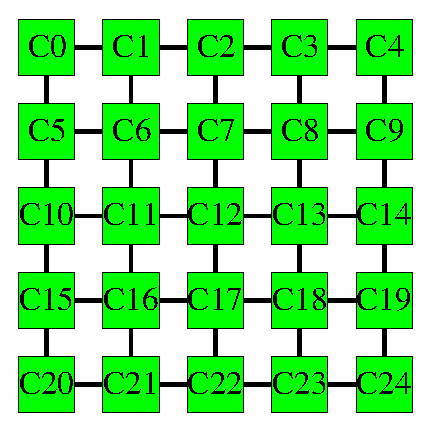
\includegraphics[scale=0.45]{figure/MeshArch.eps}
}%
\hspace{0.2cm}
\subfigure[\textbf{Hyper cube Architecture}]{%
\label{Hypercube}%
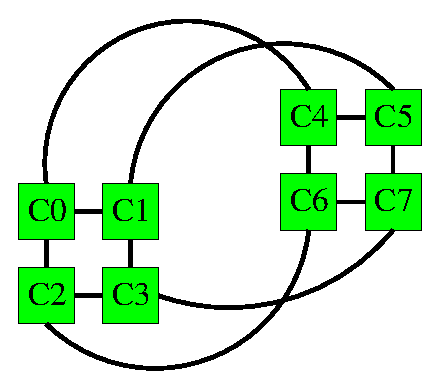
\includegraphics[scale=0.45]{figure/HyperCubeArch.eps}
}%
\hspace{0.2cm}
\subfigure[\textbf{Star Architecture}]{%
\label{Star}%
\includegraphics[scale=0.45]{figure/StarArch.eps}
}%

\end{center}
\vspace{-0.4cm}
\caption{\textbf{Multicore interconnection network}}
\label{Interconn}
\vspace{-0.3cm}
\end{figure*}


\subsection{Multiphase Application}    
Most of applications run time characteristics exhibit time varying phase behavior \cite{Cho06,Sherwood03}. 
Applications impose different performance metric values in different  time intervals. During each phase an application has same value for performance metrics. These applications running time can be partitioned in different number of  phases according to performance metrics like  {\bf Instruction level parallelism (ILP)}, {\bf Instructions per clock period (IPC)}, {\bf Number of L1 cache hits (Hits)} etc. As an example, in paper \cite{Benerjee08}, Banerjee et. al. used IPC profile to detect different phases of applications running time. They observed different benchmarks program and detected phases as shown in Table \ref{mpdetection}. 

%\begin{figure} [h]
%\centering
%\includegraphics[scale=0.5]{figure/ProcGridMXN.eps}
%\vspace{-0.2cm}\caption{\textbf{$M \times N$ processor interconnected in a mesh network}}
%\vspace{-0.3cm}
%\label{ProcGridMXN}
%\end{figure}

\begin{table} [tb]
\centering
\footnotesize
\setlength{\tabcolsep}{0.7mm}
\begin{tabular}{|c|c| |c|c| |c|c|}
\hline
\textbf{SPEC INT} & \textbf{Phases} & \textbf{SPEC FP} & \textbf{Phases} & \textbf{MEDIA} & \textbf{Phases} \\
\hline
bzip2 & 6 & ammp & 4 & mpeg2enc & 3 \\
\hline
crafty & 3 & applu & 3 & mpeg2dec & 3 \\
\hline
gcc & 6 & facerec  & 5   & cjpeg & 4 \\
\hline
gzip & 6 & equake & 6 & swim & 3 \\
\hline
mcf & 6 &  mgrid & 4   & lame & 3 \\
\hline
parser & 7 & mesa & 3 & caudio & 2 \\
\hline

\end{tabular}
\vspace{-0.1cm}\caption{Number of phases of benchmarks \cite{Benerjee08}}
\vspace{-0.3cm}
\label{mpdetection}
\end{table}

\subsection{Application scheduling and binding}

A multiphase application may have variable core requirement at various phases of its execution. If the resources are allocated without considering the variable core requirement at different phases of the application, then the system will remain underutilized. Thus, scheduling and binding strategy considering multiphase behavior plays an important role in achieving high performance and throughput. Scheduler decides the subset of tasks, the multiphase schedule of applications, which are going to be executed on the cores. After the multiphase multiprocess schedule is generated the binding algorithm comes into picture. The processor binding algorithm maps or binds the scheduled applications on the multicore system. This algorithm specifies the binding location of the core on which the task to be binded. This binding is done so that the same application's tasks are binded nearby. If the cores assigned to the same application are spread far away from each other then there will be more communication delay. So the algorithm should try to reduce the communication delay.

Other consideration while binding applications is to reduce the internal and external fragmentation on cores. Internal fragmentation occurs if more number of the cores are allocated to an application than the number of cores required. External fragmentation occurs if there are enough number of free cores to bind the task but the free cores are not continuous, thus resulting in distant binding of applications and increasing communication delay.

\subsection{Contribution and Organization}
TODO
%The main contributions of this paper are (a) a new era of scheduling and binding multi-phase applications on to mesh multicore architecture, (b) surveyed of scheduling multi-phase application (parallel chain) on to multicore architecture and their complexity, (c) Modeling task binding problem in information theoretic model, geometric model and sequence alignment model to understand the problem from different prospective and (d) also we have proposed mixed of critical path and dynamic programming methodology for scheduling multi-phase application on to multicore, and to bind scheduled application to multicore mesh architecture a viable and easy mixed of sequence alignment model and geometric model is proposed and used.


\section{Assumed Model and  Architecture} 

\subsection{Architecture model}


In this paper, we are working on cores arranged in linear architecture \ref{LinArch}. There are $n$ interconnected {\bf processing elements(PEs or cores)} $c_1,c_2,\:...,\:c_{n}$. The assumed communication infrastructure consists of a data network and a control network, each containing routers and channels connected to the cores via standard {\bf Network interfaces (NI)} as described in \cite{paper14}.  

\subsection{Assumed application model}

The applications span over multiple phases. Each phase of an application can be divided into one or more tasks. Each phase of an application may require more than one core. Each phase has two parameters associated with it. The parameters associated are number of cores that application requires in the phase and processing time to complete the phase. As shown in Fig. \ref{app_behav} application $a_1$ requires 7 cores for 4 time units in phase $t_1$, $a_2$ requires 4 cores for 3 time units in phase $t_2$. Applications $a_1$, $a_2$, $a_3$, $a_4$ has 3, 4, 2 and 5 phases respectively. The arrow represents the dependency among phases. Next phase cannot start before the previous phase has finished execution.


\begin{figure}[tb]
\centering 
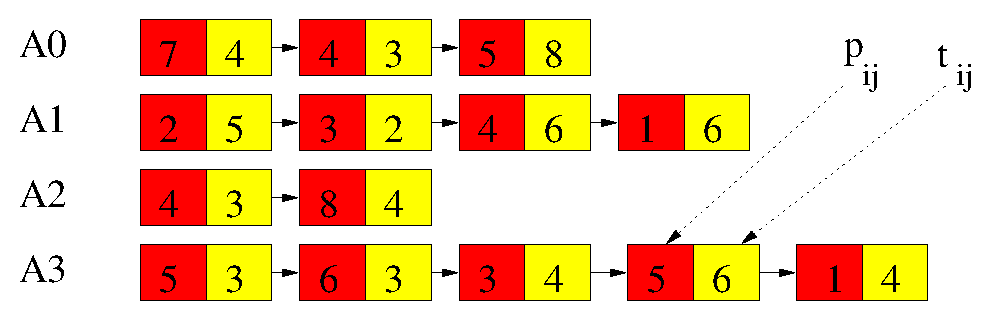
\includegraphics[scale=0.5]{./figure/AppEnv.eps}
\vspace{-0.2cm}\caption{Multi-phase running behavior of applications}
\vspace{-0.3cm}
\label{app_behav}
\end{figure}

  
Let us assume that the schedule consists of set of $m$ applications $\{a_1, a_2\:...\:, a_{m}\}$ and $k$ phases $\{t_1, t_2\:...\:,t_{k}\}$. We are given the schedule $sch$ of the applications. The core requirement in $t_i$ phase for application $a_j$ is $sch_{ij}$. The time to complete for each phase of all applications is assumed same. The total number of core requirement for any phase for all applications is less than or equal to the total number of available cores. The schedule $sch$ is mapped on the cores to get the binding $b$. The application binded in phase $t_i$ on core $c_j$ is represented by $b_{ij}$.


\subsection{Allocation model}

The main goal of mapping is to allocate the appropriate resources (number and relative position of cores to be allocated) to the incoming application tasks such that the communication cost and memory access cost is minimized.  At the same time, all the pre-existing applications still continue to run on the initial set of resources they have been allocated earlier.

\subsubsection{Data movement factor ($dmf$)}
%TODO FIGURE
This is a measure of overall movement of data during execution of the scheduled applications on multicore system.\ \\
The applications are binded on the cores in each phase. At the start of phase, cores allotted to an application read data from a specific core where the same application has written data in the previous phase. At the end of phase, cores allotted to each application chooses a core and write data to it from where the cores of the same application will read data in next phase.\ \\
The data movement overhead for a phase is defined as the sum of both reading overhead and writing overhead for that phase. So total $dmf$ is defined as sum of all data movement overheads in each phase for all the applications.\ \\
Let us consider ${t_i}^{th}$ phase in which application $a_j$ is binded at locations $\{l_1,l_2\:...\:, l_u\}$ and in ${t_{i+1}}^{th}$ phase the same application is binded at $\{l'_1,l'_2\:...\:, l'_v\}$. Now the cores of application in ${t_i}^{th}$ phase writes at location $x_i$ from which the cores of same application in ${t_{i+1}}^{th}$ phase read from. So we are minimizing the sum of squares of data movement.

\begin{figure}[tb]
\centering 
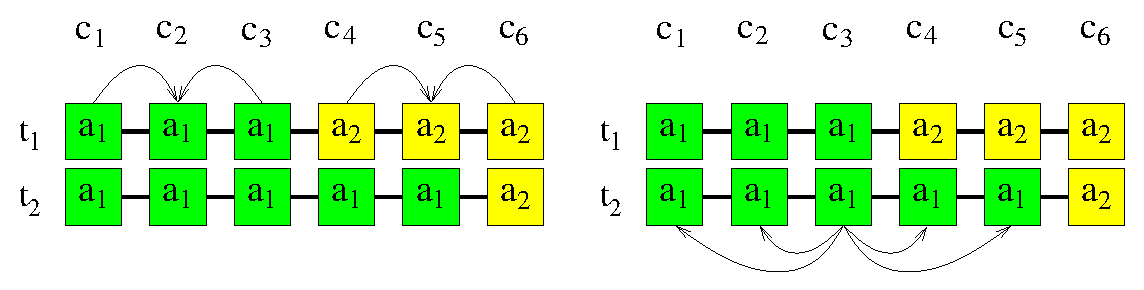
\includegraphics[scale=0.5]{./figure/dmf.eps}
\vspace{0.0cm}\caption{Data Movement Factor}
\vspace{-0.1cm}
\label{dmf}
\end{figure}

\begin{equation} 
dmf_i=\sum_{j=1}^{u}(x_i-l_j)^2+\sum_{j=1}^{v} (x_i-l'_j)^2
\label{dmfeq1}
\end{equation} 

\ \\
$l_i$ $\in$ ${1, 2\:...\:, n}$ \ \\
$l'_i$ $\in$ ${1, 2\:...\:, n}$ \ \\
and differentiating this we will get, \ \\
\begin{equation} 
x_i=\lceil(\sum_{j=1}^{u} l_i + \sum_{j=1}^{v} l'_j) /(u+v) \rceil
\label{dmfeq2}
\end{equation} 
\ \\
Substituting $x_i$ from \ref{dmfeq2} in equation \ref{dmfeq1} we will get $dmf_i$ of phase $t_i$. For phase $t_k$ there won't be any writing overhead of next phase so $dmf_k$ and $x_k$ in that case will become 
\begin{equation} 
dmf_k=\sum_{j=1}^{u}(x_k-l_j)^2
\label{dmfeq3}
\end{equation}
\ \\
\begin{equation} 
x_k =\lceil(\sum_{j=1}^{u} l_i) /u \rceil
\label{dmfeq4}
\end{equation} 
\ \\
Similarly there will be no reading overhead for $t_1$ phase and $dmf_1$ can be similarly calculated. Therefore, the total data movement factor $dmf$ can be calculated as 
\begin{equation} 
dmf = \sum_{i=1}^{k}(dmf_i)
\label{dmfeq5}
\end{equation} 
\ \\
\subsubsection{Entropy}
\begin{figure}[tb]
\centering 
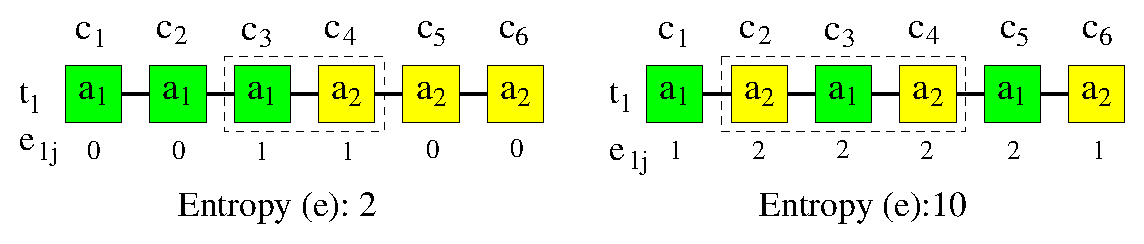
\includegraphics[scale=0.5]{./figure/entropy.eps}
\vspace{0.0cm}\caption{Entropy}
\vspace{-0.1cm}
\label{entropy}
\end{figure}

It is a measure of closeness of tasks of an appication binded on multicore system. This measure depends on the binding of tasks of an application in both same and neighboring phases.

Core Entropy $e_{ij}$ in phase $t_i$ of core $c_j$ is defined as the number of tasks assigned on neighboring cores which differs from the task assigned on the current core. Thus,
\begin{equation} 
e_{ij} = 1\left \{ b_{i,j},b_{i,j+1} \right \} + 1\left \{ b_{i,j},b_{i,j-1} \right \} + 1\left \{ b_{i,j},b_{i-1,j} \right \} + 1\left \{ b_{i,j},b_{i+1,j} \right \} 
\label{ce}
\end{equation} 
Therfore the total entopy $e$ of the binded applications is the sum of core entropies of all the cores in all phases. The equation becomes

\begin{equation} 
e = \sum_{i=1}^{k}\sum_{j=1}^{n}ce_{ij}
\label{totalentropy}
\end{equation}

\section{Previous Work}

As stated above, our problem is binding of applications on the cores in each phase. While binding the applications on phase $t_i$ we need to keep in mind the binding of the applications on the previous and the next phases for the minimization of data movement. So for minimization of overall data movement while binding the applications on the current phase we eventually need to consider the binding of applications on all the phases. While doing this for a particular application for a particular phase we may end up leaving some cores which may be filled by some other application so that identical applications are aligned in successive columns. This problem is exactly similar to {\bf multiple sequence alignment (MSA)} problem. Finding optimal solution of MSA problem is computationally difficult. This problem is already proved to be NP-complete \cite{Wang94}[7][8]. So our problem i.e. finding the optimal binding of applications on the linear architecture in multi-phase system is NP complete.
%general schedule+binding concept ...DAG graph...reference
\section{Scheduling of multiphase application on to multiprocessor}
%TODO DAG FIGURE
Scheduling is an important aspect of operating system. By this threads and processes are given access to system resources. These system resources can be processor time, communications bandwidth, memory address ranges etc. This is done to balance load to achieve a target quality of service. It helps in achieving multitasking and multiplexing. 

In general, there are multiple applications that needs execution. These applications can communicate with each other. These can share data with each other. Within one application there can be multiple inherent dependencies. An application consist of tasks with precedence constraint is modeled as a {\bf directed acyclic graph (DAG)}. DAG's nodes represent tasks of the application and directed edge represent communication or dependency between tasks. The execution of these tasks can be divided into various phases and for each phase these tasks can have multicore requirement. So for a given set of $m$ applications, these applications are divided into various sub-tasks which form the $DAG$ which is scheduled to run on a multicore system. The schedule fulfill the dependency criteria among the various processes. The schedule of processes can be seen in Fig. \ref{app_behav}. 
\section{Mapping of scheduled multiphase application on to multiprocessor}
\subsection{Mapping}
%(detail, formal definition, mapping on general architectures, communication delay, data sharing)
Mapping is another very crucial step in parallel computing paradigm. It directly effects the performance of the parallel computing system.
The objective is to find a mapping that maximizes the throughput of the system. It is a method of arranging applications on cores for their independent execution on multicore platforms. So given a schedule i.e. the applications with their core requirements in each phase, mapping of applications means arranging applications on the cores by using a mapping algorithm. Mapping of applications is largely dependent on the architecture in consideration.

\subsubsection{Communication Delay}
The architecture which has more connected cores will have less communication delay than the one having less connected cores i.e. if the communication distance between cores in one architecture is less than the communication distance between cores in the other architecture then the communication will be fast in first architecture as compared to the other architecture.
For example, Hyper cube architecture will have less communication delay as compared to linear architecture.

\subsubsection{Mapping Approaches and Optimization}
%TODO
%Let the schedule consists of set of $m$ applications $\{a_0, a_1, a_2,.., a_{m−1}\}$ and $k$ phases $\{t_0, t_1, ...,t_{k-1}\}$. The core requirement for application $a_i$ at $t_j$ phase is $p_{ij}$.There are $n$ processing elements (PEs or cores or processors) ($c_0, c_1,c_2 ...c_{n-1}$) interconnected with each other linearly.

\section{Mapping Algorithms}

%Random Algorithm
\subsection{Random Algorithm}
As shown in algorithm \ref{algrandom}, we minimize the overall entropy of the binding. We start with a random generated binding of processes to the cores. Then we calculate the initial total entropy of the binding. We randomly select a row (i.e phase) and two columns (i.e. cores on which applications are bind).We try to swap the application core binding for these chosen applications for that phase and again calculate the new total entropy($e'$) of the binding and if this $e'$ is less than e then we accept the change else we return to the previous configuration. This we do for large number of times till the value converges.This way by random swapping we are bound to get caught in some local minima or best global minima for some starting configuration. Time complexity of the algorithm is $O(m + k*n + l)$. Since $m$, $k$, $n$ and $l$ are constants, so the overall time complexity is $O(1)$. The new entropy calculation can be done in $O(1)$ time by exploiting the relation between the new entropy and the previous entropy.

\begin{algorithm}[tb]
\footnotesize
\textbf{Input:} Schedule (sch) of the processes \ \\
\textbf{Output:} Binding(b) and total entropy(e).
\begin{algorithmic}[1]
\STATE  Generate a random permutation of applications.  
\STATE  $b$ = Binding of the applications serially onto the cores in the generated order in each phase.
\STATE  $e$=  Initial entropy of the binding $b$.
\STATE  $L$ = Large number
\FOR {$i=1$ to $L$} 
\STATE Select randomly a row(r) and two columns(c1,c2).
\STATE Swap the elements b[r][c1] and b[r][c2].
\STATE $e'$ = new entropy of the binding.
\IF {$e' \leq e$} 
\STATE $e' = e$
\ELSE
\STATE Swap the elements $b[r][c1]$ and $b[r][c2]$.
\ENDIF
\ENDFOR
\STATE Output the total entropy $e$ and binding $b$.
\end{algorithmic}
\caption{\textbf{Random Algorithm for Mapping}}
\vspace{-0.1cm}
\label{algrandom}
\end{algorithm}

%Left-Right Algorithm
\subsection{Left-Right Algorithm}

\begin{figure}[tb]
\centering 
\includegraphics[scale=0.5]{./figure/left_right.eps}
\vspace{0.0cm}\caption{After Left-Right Coarse Pass Algorithm \ref{algLRP1}}
\vspace{-0.1cm}
\label{figLRP1}
\end{figure}


\begin{figure}[tb]
\centering 
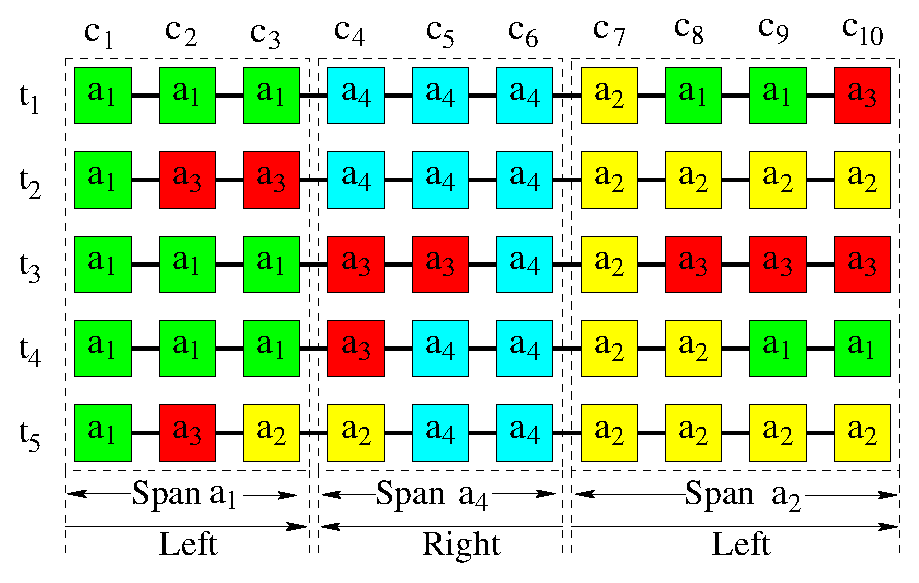
\includegraphics[scale=0.5]{./figure/left_right_fine.eps}
\vspace{0.0cm}\caption{Fine Pass \ref{algLRP2}}
\vspace{-0.1cm}
\label{figLRP2}
\end{figure}

This algorithm \ref{algLR}, uses various procedures to bind the applications on the cores. It first recognizes the applications with the highest core demand in the continous phases by calling the Biggest Block algoritm \ref{algBB}. After recognizing the biggest blocks of applications, it calculates the span of the applications (i.e. allocates some number of cores for specific applications for all the phases) by calling the Generate Span algorithm \ref{algGS}. Then we bind the applications in the span list on the cores by calling the Coarse Pass algorithm \ref{algLRP1}. The binding of the applications is done alternatively from left to right and right to left on the cores spanned by them according to the span list generated as shown in Fig. \ref{figLRP1}. According to the Fig. \ref{figLRP1}, the application $a_1$ is binded on the cores from the left to right in the span of this application. The next application $a_4$ is binded from right to left in the span. And similarly application $a_2$ is binded from left to right.The binding is done to fulfill the maximum schedule requirement of the applications for a particular phase. Then we update the free cores and the schedule of the applications that still needs to be binded. Now, we call the Fine Pass algorithm \ref{algLRP2} by passing the required parameters for binding the remaining schedule on the free cores. The applications are binded on the free cores according to the parameter $param$ passed to the function Fine Pass algorithm \ref{algLRP2}. Then the total entropy ($e$) of the binding is calculated and binding $b$ and entropy $e$ are returned.

\begin{algorithm}[tb]
\footnotesize
\textbf{Input:} Schedule $sch$, Parameter $param$ for the cost calculation \ \\
\textbf{Output:} Binding $b$, Total entropy $e$
\begin{algorithmic}[1]
\STATE list $bb$ = Biggest-Block($sch$)
\STATE list $sp$ = Generate-Span($bb$)
\STATE  ($rem\_sch$, $free\_space$, $b$) = Coarse-Pass($sch, sp, b$)
\STATE b = Fine-Pass($rem\_sch$, $free\_space$, $b$, $param$)
\STATE  $e$ = calculate total entropy of $b$
\STATE Output the total entropy $e$ and binding $b$.
\end{algorithmic}
\caption{\textbf{Left-Right Algorithm for Mapping}}
\vspace{-0.1cm}
\label{algLR}
\end{algorithm}

%Biggest Block algorithm
\subsubsection{Biggest-Block Algorithm}

\begin{figure*}[t]%
\begin{center}

\subfigure[\textbf{Biggest Blocks of $a_1$}]{
\label{imgBB1}
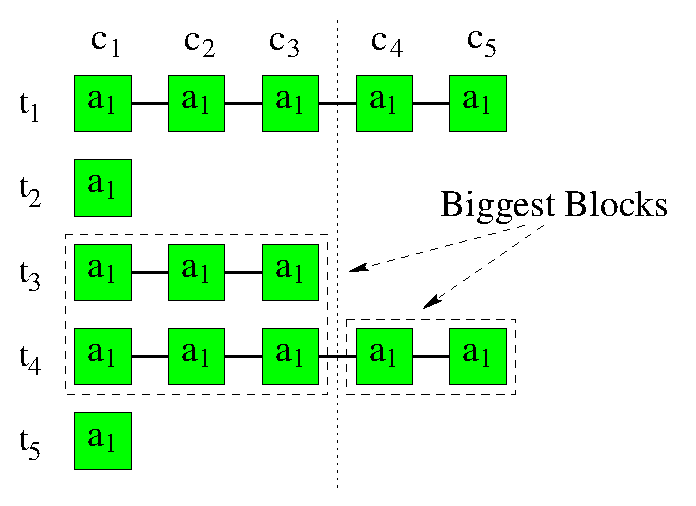
\includegraphics[scale=0.30]{figure/biggest_block_a1.eps}
}%

\hspace{0.1cm}
\subfigure[\textbf{Biggest Blocks of $a_2$}]{
\label{imgBB2}
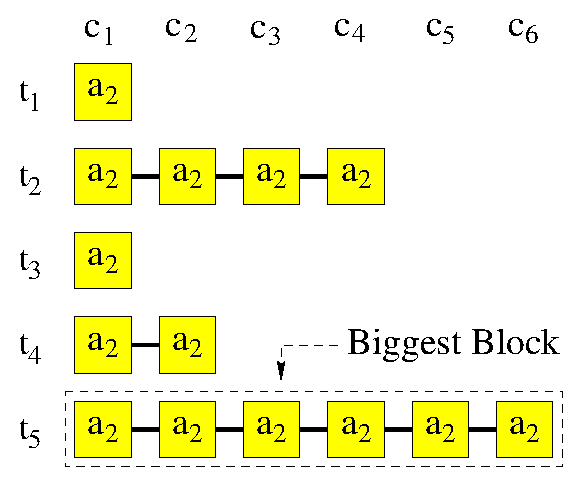
\includegraphics[scale=0.30]{figure/biggest_block_a2.eps}
}


\hspace{0.1cm}
\subfigure[\textbf{Biggest Blocks of $a_3$}]{%
\label{imgBB3}%
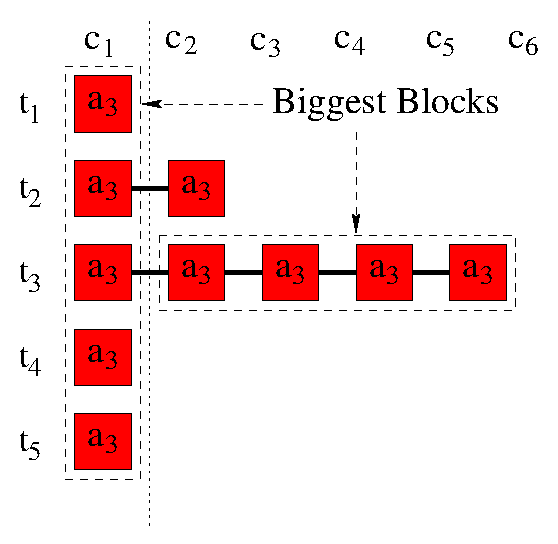
\includegraphics[scale=0.30]{figure/biggest_block_a3.eps}
}%

\hspace{0.1cm}
\subfigure[\textbf{Biggest Blocks of $a_4$}]{%
\label{imgBB4}%
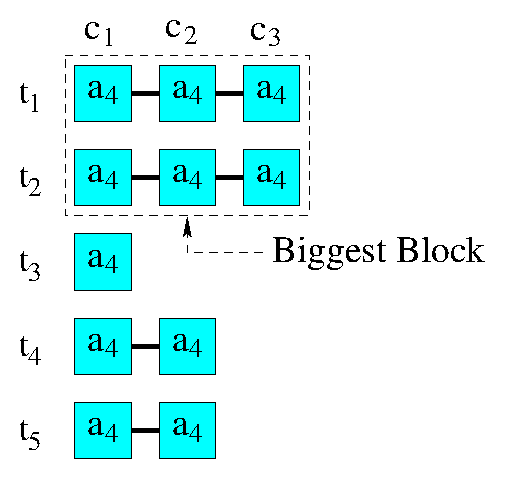
\includegraphics[scale=0.30]{figure/biggest_block_a4.eps}
}%

\end{center}
\vspace{-0.4cm}
\caption{\textbf{Biggest Blocks}}
\label{imgBB}
\vspace{-0.3cm}
\end{figure*}

This algorithm takes the schedule $sch$ as input. It breaks the core requirement of an application in the terms of big rectangular blocks whose $height$ is the phases and the $width$ is the core requirement. This way rectangular blocks are formed for each of the application and inserted in the biggest-block list $bb$. This list $bb$ is sorted according to $area$ and according to $height$ in case of tie and returned by this algorithm. 

\begin{algorithm}[tb]
\footnotesize
\textbf{Input:} Schedule $sch$ \ \\
\textbf{Output:} Biggest-Block List $bb$
\begin{algorithmic}[1]
\STATE list $bb$
\FOR{ $i$ = 1 to $m$ }
	\WHILE{ $sch_{(1:k)i}$ !=0}
		\STATE $rect$ = Calculate largest rectangle in array $sch_{(1:k)i}$
		\STATE Insert $rect$ in $bb$
		\FOR{each phase $k$}
			\STATE Subtract the width of the $rect$ from the $sch$ of the application $i$ 
		\ENDFOR	
	\ENDWHILE
\ENDFOR
\STATE Sort the list $bb$ according to area and then according to height $h$ or rectagle
\STATE Return the list $bb$.
\end{algorithmic}
\caption{\textbf{Biggest-Block}}
\vspace{-0.1cm}
\label{algBB}
\end{algorithm}

%Generate Span Algorithm
\subsubsection{Generate-Span Algorithm}
This algorithm \ref{algGS} takes the list of rectangles $bb$ returned by the Biggest-Block algorithm \ref{algBB} as input. It takes the elements from the rectangle one by one and inserts into the span list $sp$. The $rect$ is inserted in list $sp$ only if there is no already existing rectangle in the list $sp$ with same application number as of the $rect$. If there do exists a rectangle in the list $sp$ with same application number as of the $rect$,then the $span$ of the $elem$ in the list $sp$ is increased by the $width$ of the $rect$. While inserting the elements in the list $sp$, we keep in mind that sum of the span of all the elements in the list $sp$ is less than or equal to the total number of available cores $n$. 

\begin{algorithm}[tb]
\footnotesize
\textbf{Input:} List of rectangles $bb$\ \\
\textbf{Output:} Span list of applictions $sp$
\begin{algorithmic}[1]
\STATE list $sp$
\FOR{ each rect in $bb$ }
	\IF{$rect.id$ exists in $sp$}
		\IF{$cores$ left unassigned}
			\STATE Increase the $cores$ alloted ($span$) of the $rect.id$ in list $sp$ by minimum of $cores$ remaining or $rect.height$
		\ELSE
			\STATE break
		\ENDIF
	\ELSE
		\STATE Insert the $rect$ in the list $sp$ with $span$ equal to minimum of $cores$ remaining or $rect.height$
	\ENDIF
\ENDFOR
\STATE Return the list $sp$.
\end{algorithmic}
\caption{\textbf{Generate-Span}}
\vspace{-0.1cm}
\label{algGS}
\end{algorithm}

%Phase-One of Coarse-Pass Algorithm
\subsubsection{Coarse-Pass Algorithm}
This algorithm \ref{algLRP1} takes schedule of applications $sch$, span list $sp$ to output the bind the applications $b$. This algorithm \ref{algLRP1} forms the procedure for Left-Right algorithm \ref{algLR}. It binds the applications on the cores, according to their $span$ in span list $sp$ and maximally satisfies the $core$ requirement at each phase. The binding for the applications at odd postion in the span list($sp$) is done from left to right starting from the $elem.start$ to $elem.end$ where $elem$ is the element in the span list($sp$) as shown in Fig. \ref{figLRP1}. Similarly for the applications at even position in the span list($sp$) the binding is done from right to left starting from the $elem.end$ to $elem.start$ as shown in Fig. \ref{figLRP1}. The objective of binding this way is to maximize the space in the middle of two consecutive binded applications. This ways the applications can be binded together in the next binding phase by Fine-Pass algorithm \ref{algLRP2}.After binding the elements to the cores, the schedule $sch$, binding $b$ and free cores$free\_space$ is updated and outputted.

\begin{algorithm}[tb]
\footnotesize
\textbf{Input:} Schedule $sch$, span list $sp$ \ \\
\textbf{Output:} remaining schedule $rem\_sch$, the continuous free space $free\_space$ between the two binded applications, binding $b$
\begin{algorithmic}[1]
\STATE  $prev$ = 0
\FOR {each $elem$ in $sp$} 
\STATE $elem.start$ = $prev$+1; $elem.end$ = $elem.start$ + $elem.height$
\STATE $prev$ = $elem.end$
\ENDFOR    
\FOR {$i$ = 1 to $size$ of $sp$} 
\IF { i mod 2==1 } 
\STATE Bind the application on the cores from $sp[i].start$
\ELSE   
\STATE Bind the application on the cores from $sp[i].end$
\ENDIF
\STATE $free\_space$ = free cores in the bind in the each phase.   
\STATE $rem\_sch$ = schedule remaining after binding initially.
\ENDFOR
\STATE Output $rem\_sch$, $free\_space$ and $b$
\end{algorithmic}
\caption{\textbf{Coarse-Pass}}
\vspace{-0.1cm}
\label{algLRP1}
\end{algorithm}

%Phase Two Left-Right and Center-Center Algorithm
\subsubsection{Fine-Pass}
This algorithm \ref{algLRP2} takes remaining schedule $rem\_sch$, continuous free space $free\_space$ between the two binded applications, parameter $param$ and binding $b$ after Coarse-Pass algorithm \ref{algLRP1} as input. It calculates the $value_{i,j}$ when the application$a_i$ is binded in the $free\_space_j$. This $value_{i,j}$ comprises of the two cost parameters namely undershoot value($u_{i,j}$) and overshoot value($o_{i,j}$). \ \\
The undershoot value for a phase is the $\alpha$ times the space that remains unallocated while binding the application $a_i$ in the continuous block of $free\_space_j$ at phase $t_k$. Thus undershoot value $u_{i,j}$ is the summation of the total unbinded space while binding the application($a_i$) at the continuus $free\_space_j$.

\begin{equation} 
u_{i,j} = \sum\limits_{l=1}^k \alpha*(space[k]-app[k])
\label{undershoot}
\end{equation}
if ($space[k]$ - $app[k]$ $\geq$ 0 else 0) , here $\alpha$ = $param$ 
Similarly, overshoot value $o_{i,j}$ for a phase is defined as the $\beta$ times the schedule($rem\_sch_{i,k}$) that remains unbinded while binding the application $a_i$ in the continuous block of $free\_space_j$ at phase $t_k$. Thus overshoot value $o_{i,j}$ is the summation of the total unbinded schedule while binding the application $a_i$ at the continuus free space ($j$).\ \\
\begin{equation} 
o_{i,j} = \sum\limits_{l=1}^k \beta*(app[k]-space[k])
\label{overhoot}
\end{equation}
if ($space[k]$ - $app[k]$ $\geq$ 0 else 0) , here $beta = 1- param$
Therfore, Fitting Cost $fc_{i,j}$ can be calculated as \ \\
\begin{equation} 
fc_{i,j} = u_{i,j} + o_{i,j}
\label{fittingcost}
\end{equation}
This way we find the cost $fc_{i,j}$ for each application $a_i$ at each $free\_space_j$.For particular $free\_space_j$, the application $a_i$ with minimum value($fc_{i,j}$) is binded on the $free\_space_j$. This is done for all the $free\_space$. This whole process is repeated till all the applications are successfully binded on all the $free\_spaces$. After this we output the final binding $b$.

\begin{algorithm}[tb]
\footnotesize
\textbf{Input:} $rem\_sch$ remaining schedule left yet to be binded, $free\_space$ it maps the continuous free space between the two binded applications, $param$, and  $b$ binding
\textbf{Output:} $b$ the final binding of applications on cores
\begin{algorithmic}[1]
\STATE $\alpha$ = $param$, $\beta$ = $1-param$
\FOR {each $Apps$ in $rem\_sch$} 
\FOR {each space in free\_space} 
\STATE value[app][space] = 0
\FOR {for phase in range [1,k]}
\IF {space[phase] - app[phase] >= 0} 
\STATE value[app][space] += alpha*(space[phase] - app[phase])
\ELSE   
\STATE value[app][space] += beta*(app[phase]-space[phase] )
\ENDIF
\STATE Assign the not alloted application with minimum value to the free\_space
\STATE Bind the Apps alloted to the the free\_space on the cores according to the schedule for each phase
\STATE Update $free\_space$, bind, $rem\_sch$ 
\ENDFOR
\ENDFOR
\ENDFOR
\STATE Output $rem\_sch$, $free\_space$ and $b$
\end{algorithmic}
\caption{\textbf{Fine\_Pass}}
\vspace{-0.1cm}
\label{algLRP2}
\end{algorithm}

\subsection{Center-Center Mapping Algortihm}
\begin{figure}[tb]
\centering 
\includegraphics[scale=0.5]{./figure/center_center.eps}
\vspace{0.0cm}\caption{After Center-Center Coarse Pass }
\vspace{-0.1cm}
\label{figCCP1}
\end{figure}
This algorithm \ref{algCCP1} is quite similair to the previous algorithm discussed i.e. left-right algorithm \ref{algLR}. The only major difference between the two algorithm comes in the phase one of the binding of the applications on the cores. In left-right algorithm \ref{algLR}, in phase one of binding the consecutive applications were binded in the left to right and right to left fashion. But in this algorithm, the applications are binded within the span it covers on the cores starting from the middle as shown in Fig \ref{figCCP1}. That is the binding of the application on the cores in the span is middle aligned. This is done for all the applications. After this we update the free cores and calculate the remaining scheule of applications. Then as in the previous algorithm \ref{algLR}, we bind the remaining schedule on the $free\_space$ of cores by the fine-pass algorithm \ref{algLRP2}. Calculation for the total entropy $e$ is done. Then the entropy value $e$ and binding $b$ are outputted.

\begin{algorithm}[tb]
\footnotesize
\textbf{Input:} Schedule $sch$, Parameter $param$ for the cost calculation \ \\
\textbf{Output:} Binding $b$, Total entropy $e$
\begin{algorithmic}[1]
\STATE list $bb$ = Biggest-Block($sch$)
\STATE list $sp$ = Generate-Span($bb$)
\STATE  ($rem\_sch$, $free\_space$, $b$) = Coarse-Pass-Center($sch, sp, b$)
\STATE b = Fine-Pass($rem\_sch$, $free\_space$, $b$, $param$)
\STATE  $e$ = calculate total entropy of $b$
\STATE Output the total entropy $e$ and binding $b$.
\end{algorithmic}
\caption{\textbf{Center-Center Algorithm for Mapping}}
\vspace{-0.1cm}
\label{algCC}
\end{algorithm}


\subsubsection{Coarse Pass Center}
This algorithm \ref{algCCP1} takes schedule of applications $sch$, span list $sp$ to bind the applications on the binding $b$. This algorithm is specific to the Center-Center algorithm \ref{algCC}. This algorithm is similar to the previous Coarse Pass \ref{algLRP1} used in Left-Right algorithm \ref{algLR}. This algorithm \ref{algCCP1} binds the applications on the binding($b$). The binding is done according to the information in the span list($sp$). The binding of the application is on the cores is center aligned done in the span for that particular application dictated by the span list($sp$) as shown in Fig. \ref{figCCP1}. This is done for all the applications in the span list $sp$, considering the schedule $sch$ of the application. After the initial phase of binding the new values of remaining schedule $rem\_sch$, free cores $free\_space$ are calulated. This algorithm thus outputs the schedule $sch$, binding $b$ and free cores $free\_space$.
\begin{algorithm}[tb]
\footnotesize
\textbf{Input:} Schedule $sch$, span list $sp$ \ \\
\textbf{Output:} remaining schedule $rem\_sch$, the continuous free space $free\_space$ between the two binded applications, binding $b$
\begin{algorithmic}[1]
\STATE  $prev$ = 0
\FOR {each $elem$ in $sp$} 
\STATE $elem.start$ = $prev$+1; $elem.end$ = $elem.start$ + $elem.height$
\STATE $prev$ = $elem.end$
\ENDFOR    
\FOR {$i$ = 1 to $size$ of $sp$} 
\STATE Bind the application on the cores in the middle of the span from $sp[i].start$ to $sp[i].end$ fulfilling the scheule $sch[i]$ requirement.
\STATE $free\_space$ = free cores in the bind in the each phase.   
\STATE $rem\_sch$ = schedule remaining after binding initially.
\ENDFOR
\STATE Output $rem\_sch$, $free\_space$ and $b$
\end{algorithmic}
\caption{\textbf{Coarse-Pass Center }}
\vspace{-0.1cm}
\label{algCCP1}
\end{algorithm}

% Blossom weight
\begin{algorithm}[tb]
\footnotesize
\textbf{Input:} Schedule $sch$ of the processes, application $a_i$, application $a_j$  \ \\
\textbf{Output:} Weight $w$ between application $a_i$ and application $a_j$.
\begin{algorithmic}[1]
\STATE $avgI$=Average cores requirement of application $i$
\STATE $avgJ$=Average cores requirement of application $j$
\STATE $weight$=0
\FOR {p in range(0,$k$)} 
\STATE $weight + = (sch[p][i]-avgI)*(sch[p][j]-avgJ)$
\ENDFOR
\STATE return $weight$
\end{algorithmic}
\caption{\textbf{Blossom\_Weight}}
\vspace{-0.1cm}
\label{algWeightCalculation}
\end{algorithm}

\begin{figure}[tb]
\centering 
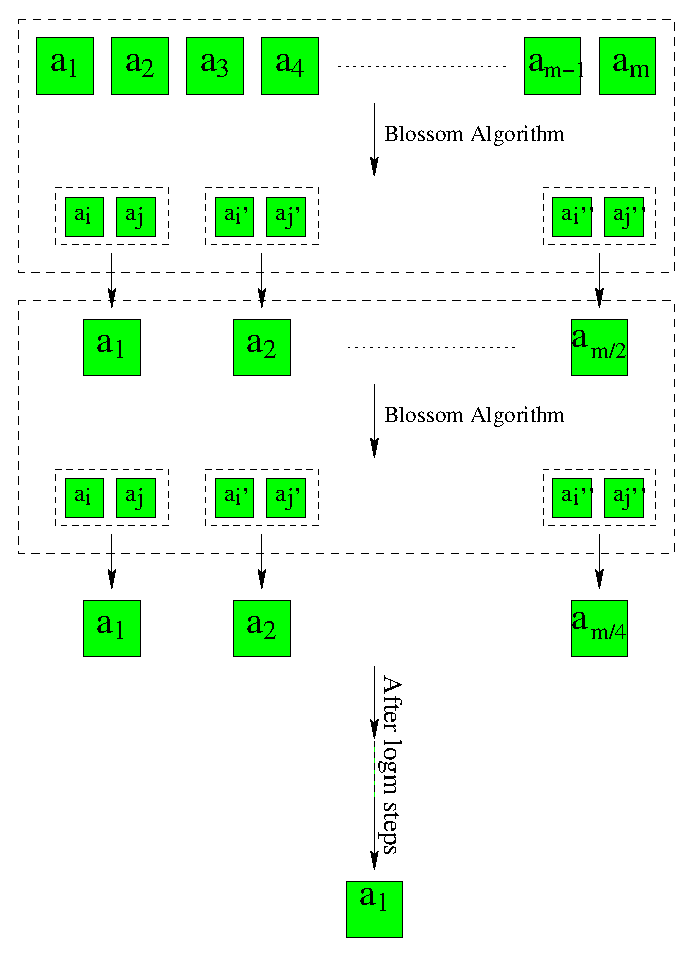
\includegraphics[scale=0.5]{./figure/blossom.eps}
\vspace{0.0cm}\caption{Modified Blossom}
\vspace{-0.1cm}
\label{blossom}
\end{figure}

%Modified Blossom
\subsection{Modified Blossom}
The algorithm \ref{algBlossom} takes scheduling innformation of applications as input. It first tries to find the application order as well as application pairs such that if the applications are binded using this information will give a better binding. We first find the application pairs. For this we first convert the sheduling information into a graph. In graph, nodes will represent applications and weighted edges represent the compatibility score between two applications. Less the compatibility score will mean more the compatibility. We are using Blossom algorithm for finding minimum cost perfect matching. The output of blossom algorithm will be the pairs of applications such that total cost is minimized in perfect matching. We store the pair information which we will use for finding the application order. We then modify the scheduling information. For it, we will assume both the applications in pair information as a single application and again find the graph and run Blossom algorithm. We do this until the applications count comes down to 1. Let say the application order we got from above be $\{a_1, a_2\:...\:, a_{m}\}$. And let say pairs P be $\{(a_1,a_2),(a_3,a_4)\:...\:, (a_{m-1},a_{m})\}$. Then for each pair in P we find the minimum processor requirement $minpairReq$ of them if they are binded toogether and bind that pair in $minpairReq$ cores. Binding is represented as k*n matrix. We will see that we have used more cores i.e. columns in binding matrix than the actual given number. Remove the extra columns in which the binding is least and bind those applications in the phases wherever the cores are not used in linear fashion starting from first column. The new binded matrix after adjusting of columns will be the final binding matrix.


%Blossom Weight
\subsubsection{Blossom Weight}
The algorithm \ref{algWeightCalculation} finds the weight between two applications using the scheduling information. We are using this algorithm while making edges between nodes while we are converting the scheduling information into a graph. We find the average cores requirement of $a_i^{th}$ and $a_j^{th}$ application and store it into $avgI$ \& $avgJ$ respectively. So the weight between two applications is calculated as product of how much extra both applications require than their average requirement. Weight will be the sum of the above calculated product in each phase.

\begin{algorithm}[tb]
\footnotesize
\textbf{Input:} Schedule $sch$ of the applications  \ \\
\textbf{Output:} Binding $b$ and total entropy $e$
\begin{algorithmic}[1]
\WHILE {$No\_Of\_Applications\_in\_Schedule$!=1}
\FOR {all ($a_i$,$a_j$) pair} 
\STATE $Edge\_Weight\_Between\_a_i\_and\_a_j$=$Blossom\_Weight(sch,a_i,a_j)$
\ENDFOR
\STATE Construct graph $G$=(applications,edges)
\STATE $perfect\_matched\_edges$=$Blossom\_Algorithm(G)$
\STATE Store the $perfect\_matched\_edges$ information
\STATE new\_schedule=after merging schedule corresponding to the applications $a_i$ \& $a_j$ if ($a_i$,$a_j$) $\in$ $perfect\_matched\_edges$
\ENDWHILE
\STATE The stored information will give the sequence $\{a_1, a_2\:...\:, a_{m}\}$ in which the applications should be binded.
\STATE $pairs$=$\{(a_1,a_2),(a_3,a_4)\:...\:, (a_{m-1},a_{m})\}$
\FOR {($a_i$,$a_j$) in $pairs$}
\STATE $minpairReq[ij]$=Minimum\_cores\_needed to bind $a_i^{th}$ \& $a_j^{th}$ applications together
\STATE $initialBinding$=$initialBinding$ + (bind $a_i^{th}$ and $a_j^{th}$ applications in minpairReq[ij] alloted cores in each phase)
\ENDFOR
\STATE $extraColumns$=$Number\_Of\_Columns\_Used$-$n$
\STATE $finalBinding$=Remove $extraColumns$ which are least binded and bind them linearly
\STATE return $finalBinding$
\end{algorithmic}
\caption{\textbf{Modified\_Blossom}}
\vspace{-0.1cm}
\label{algBlossom}
\end{algorithm}


%Figures for the algorithms
\iffalse
%Example Schedule figure
\begin{figure} [tb]
\centering
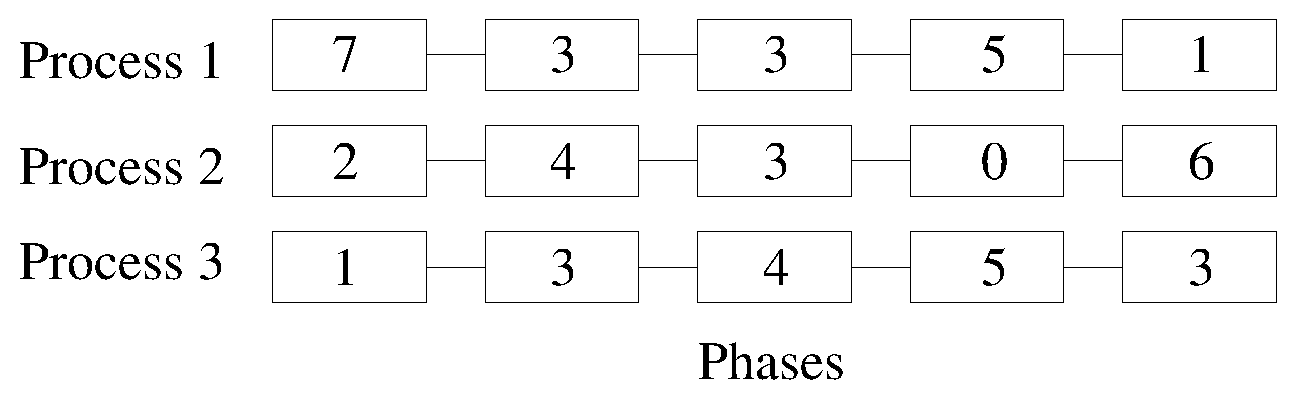
\includegraphics[scale=0.25]{figure/schedule.eps}
\caption{\textbf{Example Schedule}}
\label{imgschd}
\end{figure}

%Random Random Image
\begin{figure} [tb]
\centering
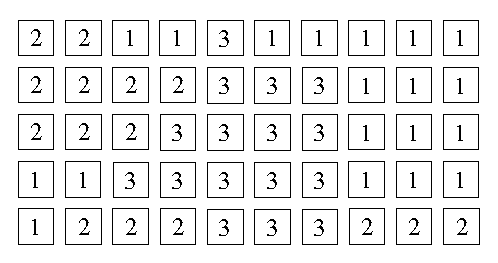
\includegraphics[scale=0.45]{figure/random_shuffle.eps}
\caption{\textbf{Binding after Random Algorithm(\ref{algrandom}) }}
\label{imgrandom}
\end{figure}

%Phase One Left-Right Image
\begin{figure} [tb]
\centering
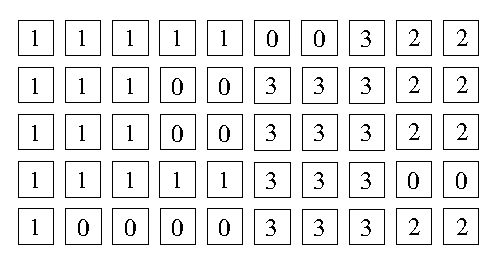
\includegraphics[scale=0.45]{figure/phase_one_left_right.eps}
\caption{\textbf{After Phase-One Algorithm(\ref{algLRP1}) used in Left-Right Algorithm(\ref{algLR}) }}
\label{imgLRP1}
\end{figure}

%Phase One Left-Right Image
\begin{figure} [tb]
\centering
\includegraphics[scale=0.45]{figure/phase_two_left_right.eps}
\caption{\textbf{Binding After Phase-Two Algorithm(\ref{algLRP2}) used in Left-Right Algorithm(\ref{algLR}) }}
\label{imgLRP2}
\end{figure}

%Phase One Center-Center Image
\begin{figure} [tb]
\centering
\includegraphics[scale=0.45]{figure/phase_one_center_center.eps}
\caption{\textbf{After Phase-One-Center Algorithm(\ref{algCCP1}) used in Center-Center Algorithm(\ref{algCC}) }}
\label{imgCCP1}
\end{figure}

%Phase One Center-Center Image
\begin{figure} [tb]
\centering
\includegraphics[scale=0.45]{figure/phase_two_center_center.eps}
\caption{\textbf{After Phase-Two Algorithm(\ref{algLRP2}) used in Center-Center Algorithm(\ref{algCC}) }}
\label{imgCCP2}
\end{figure}
\fi

\section{Experiment and result}

\ \\ 
(2 PAGE, GRAPH, AND IT'S EXPIATION, WHY ONE PERFORMS BETTER AND OTHER DOESN'T, IMPLEMENTATION DIFFERENCE AND WHY ONE ALGO IS BETTER, INTERPRETATION OF CONCLUSION) \ \\
The graphs in the Figure ~\ref{EntropyVsProc}, Figure ~\ref{EntropyVsPhases} and Figure ~\ref{EntropyVsApps} shows the variation of total entropy with the variation in number of processors, phases and phases by running the various algorithms described in this paper on the multiphase schedule. The red line in the graphs indicate the initial entropy. This value is calulated by binding the multiphase schedule on the cores by generating any random permutation of applications and binding them on the cores in the linear fashion. This is the initial entropy value and is the highest for all the data points. This highest entropy value indicates that the binding of schedule on the cores in not efficient. \ \\

The plot of Random Algorithm(\ref{algrandom}) is shown with the green line. In this algorithm after binding the schedule on the cores in the random manner, we minimzed the entropy value by swapping the applications on the cores for a particular phase. This process of swapping the applications on cores was again done randomly for the phases and for the cores in a particular phase. This random swapping was done for a large number of times accepting the swap if the new entropy value was lower than the previous value. This algorithm leads to the low values of overall total entropy. This algorithm has a drawback i.e. it may not always give the optimal minimum value of total entropy. As the initial starting binding is random and this plays a significant roles in the subsequent random swaps. By this the state may be trapped in the local minima and the configuration of binding never changes. This local minima problem is serious and this is what happens, hence the carefully devised algorithm may give better results than the Random Algorithm \ref{algrandom}. \ \\

The total entropy value of Left-Right Algorithm(\ref{algLR}) is in between the total initial entropy value and the total entropy value after applying Random Algorithm(\ref{algrandom}). In this algorithm, the binding was done in the two crucial phases. In the phase phase of the binding the biggest continuous rectangular application blocks in the continuous phases were recognized. After recognizing these biggest blocks, span(cores) for the applications with the highest area were allocated till all the cores gets spanned. Then the binding on the spanned cores was done by the applications according to the schedule.This phase may lead to some free cores in some of the phases and schedule of some application unsatisfied. To bind the remaining schedule, we call the Phase-Two Algorithm(\ref{algLRP2}). This algorithm takes the parameter($param$). This parameter is used in calculating the cost values while assigning the free cores to the remaining schedule. By using this $param$ value we calculate the undershoot parameter($alpha$) and overshoot parameter($beta$). The undershoot parameter($aplha$) is responsible for taking in account the penalty for the free cores left(internal fragmentation) while binding the application in the continous free space between the two consecutive applications binded in phase one. The overshoot parameter($beta$) penalizes for the schedule of the application that still is unsatisfied after binding the application in the free space between the two consecutive applications binded in phase one. We want to minimize the overall penalty. The application best-fitted in the free spaces. This results shown in the graphs are when parameters $alpha$ and $beta$ are given equal weightage. This way the remaining schedule is binded to the cores and the overall entropy value is calculated. This algorithm performs slighty better than Center-Center Algorithm(\ref{algCC}) but significantly reduces the intial value of the entropy. We can apply the Random Algorithm(\ref{algrandom}) over the binding we got from this alogrithm as the initial configuratiom. This way we can further minimize the overall total entropy of the binding.\ \\

The results of the Center-Center algorithm(\ref{algCC}) are comparable to the results of the Left-Right algorithm \ref{algLR}. This algorithm also binds the schedule in the two phases. This algorithm differs from the Left-Right algorithm(\ref{algLR}) just in the phase one of the binding. In phase one of the algorithm the binding is done by calling the Phase-One-Center Algorithm(\ref{algCCP1}). It center binds the applications in the cores spanned by them. The binding in second phase is done by calling the Phase-Two algorithm(\ref{algLRP2}). This also considers the undershoot($alpha$) and overshoot parameter($beta$) values while binding. By running Random Algorithm(\ref{algrandom}) over the binding outputted by this algorithm, the total entropy value can be further improved.  \ \\

The results of Modified Blossom algorithm(\ref{algBlossom}) is far better than Left-Right algorithm \ref{algLR} and Center-Center algorithm(\ref{algCC}). This algorithm performs better than the random algorithm also. The main crux of the algorithm lies in extracting the application order as well as application pairs such that if the applications are binded using this information will give a good binding. The algorithm uses Blossom Algorithm (provide reference) logm times to find the application order. After finding the application order the binding step is simple. We bind the applications in pair according to the application order that we got from above. Since this algorithm binds considering a more strong form of closeness between applications, this algorithm performs best among the available algorithms.

\begin{figure} [tb]
\centering
\includegraphics[scale=0.45]{figure/data1.eps}
\caption{\textbf{Variation of entropy with processors}}
\label{EntropyVsProc}
\end{figure}

\begin{figure} [tb]
\centering
\includegraphics[scale=0.45]{figure/data2.eps}
\caption{\textbf{Variation of entropy with Phases}}
\label{EntropyVsPhases}
\end{figure}

\begin{figure} [tb]
\centering
\includegraphics[scale=0.45]{figure/data3.eps}
\caption{\textbf{Variation of entropy with Applications}}
\label{EntropyVsApps}
\end{figure}

Figure ~\ref{EntropyVsProc}. is shows Variation of entropy with processors. Figure ~\ref{EntropyVsPhases}. is shows Variation of entropy with number of phases. Figure ~\ref{EntropyVsApps}. is shows Variation of entropy with number of application.

\section{Conclusions and Future Work} \label{concl}
The minimum value of total entropy is obtained by running the blossom algorithm to bind the given schedule. Left-Left Algorithm (\ref{algLR}) and Center-Center Algorithm(\ref{algCC}) gives the average resutls between the initial entropy value and the total entropy value obtained by running the Blossom algorithm.
\bibliographystyle{IEEEtran}
%\setstretch{0.68}
%\bibliographystyle{unsort}
%\footnotesize
%\normalsize
\bibliography{MPBind}
\end{document}

